% !TeX root = ../main.tex

\chapter{Future work}
\label{chapter:future_work}
This chapter describes, what further work can be done on Isabelle/VSCode by later projects.

\section{Features}
Although several new features have been added throughout this project, there is still some work to be done, so that the functionality offered in Isabelle/VSCode is comparable to that of jEdit.  In this section, we will explore new features which could be added, to improve the overall user experience. 

\subsection{Shared Server Instance}
When working with multiple instances of VSCode, each of them will start their own Isabelle/VSCode server. This has the following disadvantages:
\begin{itemize}
    \item As we stated in \Cref{section:startup}, the startup of the server takes a considerable amount of time. The user would have to wait out the server every time a new VSCode window is opened.
    \item Each server instance requires a lot of resources, especially memory.  This makes working, with multiple VSCode windows, on low memory machines impossible. 
\end{itemize}

In the future, it would be beneficial to have the client attach to an already running server instance. Implementing this feature would take some effort since the server would have to be refactored to support requests from different VSCode instances.

\subsection{Manual Workspace Setup}
With the new changes, the extension gets activated only when there is a ROOT file in the current directory. This stops users from working outside of such directories, without sessions. There are some cases where it is advantageous for the user to work without a session. In this case, the user would set up an empty workspace and then add the theories he needs to work with. All these theories would be added to the \texttt{Draft} session since the workspace was set up without a session. 

To implement this feature the following steps need to be taken:
\begin{enumerate}
    \item Add a new command to the extension, which triggers the setup of a workspace, without needing a ROOT file.
    \item Give the server an option to start without the current directory.
    \item Refactor the Isabelle file system to support starting without getting the sessions from the server.
\end{enumerate}

This feature would be beneficial to users who only want to make quick edits and are not interested in the session structure of the project.

\subsection{Proper Formatting for State/Output}
In \Cref{section:state-panel}, we added the syntax highlighting for the panels. A problem that came up, was the incorrect formatting of the text in the state and output panels. The line breaks in the \texttt{WebViews} are missing and need to be added in the correct positions.

\subsection{Extra Semantic Editor Perspectives}
Not all semantic editor perspectives that are present in jEdit can be found in VSCode. Until now, only the state and output perspective have been implemented. From the missing perspectives, the most important are:
\begin{itemize}
    \item \textbf{Sledgehammer.} This perspective is helpful for invoking the Isar \texttt{sledgehammer} command. This command applies automatic theorem provers on the current proof goal.
    \item \textbf{Query.} This perspective gives the user the possibility to request extra information from the prover.
\end{itemize}

The jEdit interfaces of these panels can be easily replicated in VSCode since all the necessary GUI elements are already available.

% \begin{figure}[htb]
%     \centering
%     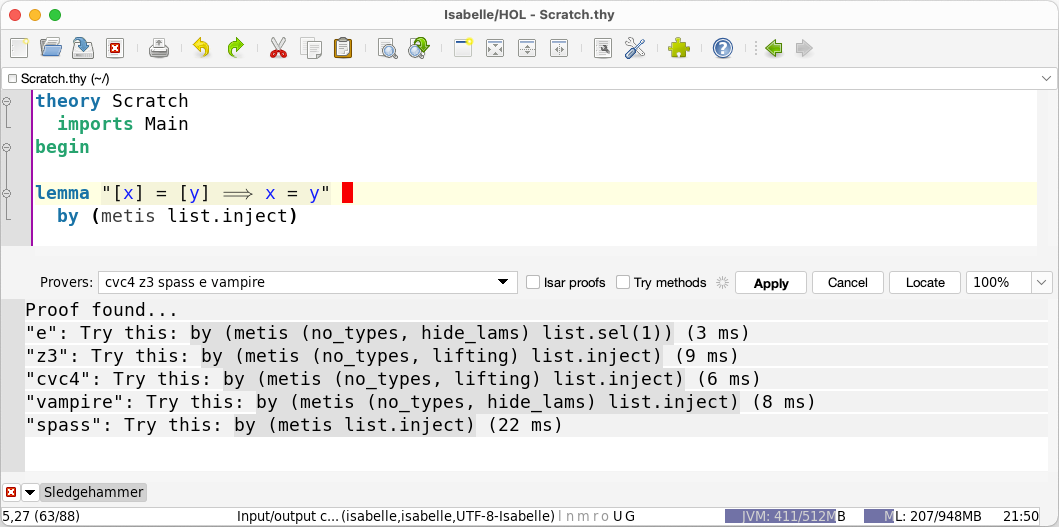
\includegraphics[width=0.8\textwidth]{figures/future/sledgehammer.png}
%     \caption{jEdit interface of the sledgehammer panel~\parencite{jedit}.}
%     \label{fig:sledgehammer_panel}
% \end{figure}

% \begin{figure}[htb]
%     \centering
%     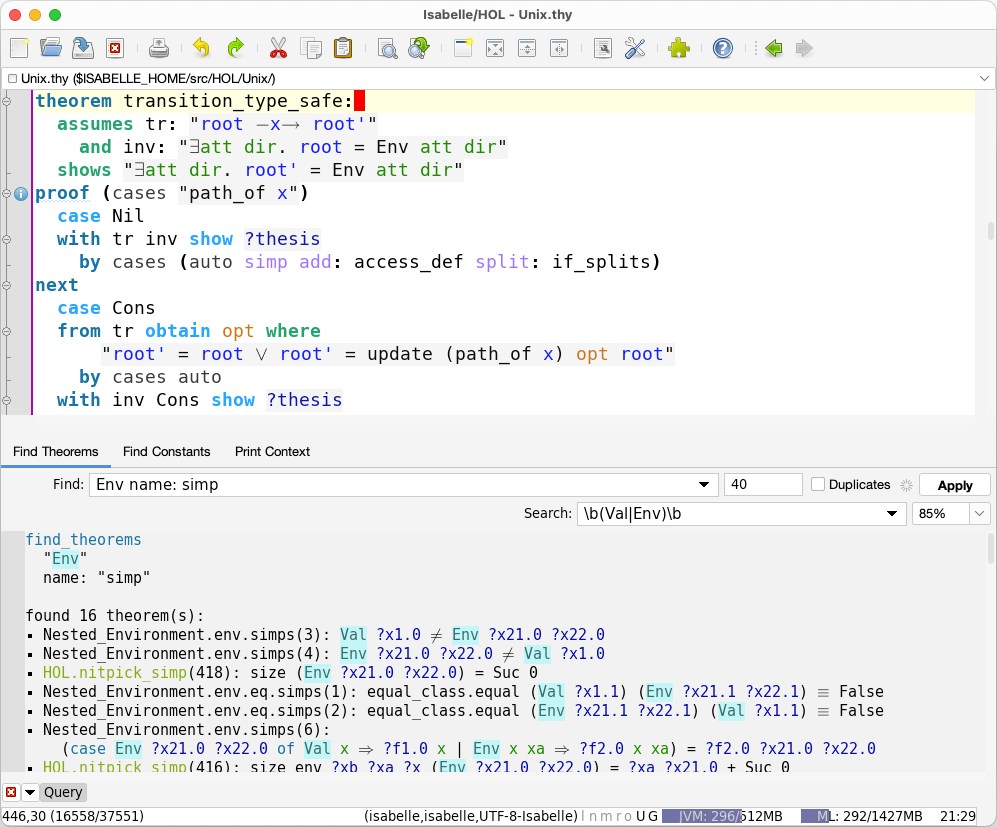
\includegraphics[width=0.8\textwidth]{figures/future/query.png}
%     \caption{jEdit interface of the query panel~\parencite{jedit}.}
%     \label{fig:query_panel}
% \end{figure}


\section{Additional Code Editors and IDEs}
The use of a language server makes it possible to quickly develop plugins for other code editors and IDEs, which also use the Language Server Protocol. Furthermore, the language server of Isabelle/VSCode uses the standard endpoints of the protocol for most communications. This should reasonably speed up the development of such plugins.   Normally, most editors require some level of customization in order to work properly. Below, we will explore the code editors most suitable for an Isabelle plugin, given the current state of the language server.

\subsection{Sublime Text}
\emph{Sublime Text} is a sophisticated text editor for code, markup and prose~\parencite{sublime}. The Language Server Protocol is already fully integrated into Sublime Text~\parencite{lsp_sublime}. This, along with its popularity (see \autoref{fig:editors_pop}), makes Sublime Text a good candidate for an Isabelle plugin.

In its current state, the language server would only provide the basic language features. More complicated features would still have to be implemented. One advantage of using Sublime Text is that there wouldn't be a need to implement a separate file system, as was necessary for the VSCode extension. Similar to jEdit, in Sublime Text, an encoding can be added programmatically from within a plugin. This makes developing a plugin for this editor, easier in comparison to VSCode.

\subsection{IntelliJ IDEA}
\emph{IntelliJ IDEA} is an integrated development environment written in Java~\parencite{intellij}. We mentioned in \Cref{section:isabelle} that Scala is used to develop the systems around the Isabelle environment. IntelliJ IDEA is one of the preferred IDEs for developers to work with Scala. The language is fairly supported in IntelliJ through a plugin. 

It could be feasible in the future to support a plugin for Isabelle in IntelliJ. This would be helpful for users who are already working on Isabelle/Scala with this IDE. Then IntelliJ would become a fully-featured IDE for working with Isabelle. A user wouldn't need to have an instance of jEdit or VSCode running alongside an IntelliJ instance. All operations could be conducted within only one IDE.

The Language Server Protocol is not natively supported in IntelliJ. This is potentially a big hurdle to developing the plugin for IntelliJ, but there is already a highly rated third-party plugin that adds support for the protocol~\parencite{intellij_lsp}.